% !TeX spellcheck = en_US
%% 字体:方正静蕾简体
%%		 方正粗宋
\documentclass[a4paper,left=2.5cm,right=2.5cm]{article}

\usepackage[utf8]{inputenc}
\usepackage{fontspec}
\usepackage{cite}
\usepackage{xeCJK}
\usepackage{indentfirst}
\usepackage{titlesec}
\usepackage{longtable}
\usepackage{graphicx}
\usepackage{float}
\usepackage{rotating}
\usepackage{subfigure}
\usepackage{tabu}
\usepackage{amsmath}
\usepackage{setspace}
\usepackage{amsfonts}
\usepackage{appendix}
\usepackage{listings}
\usepackage{xcolor}
\usepackage{geometry}
\setcounter{secnumdepth}{4}
\titleformat*{\section}{\LARGE}
\renewcommand\refname{参考文献}
%\titleformat{\chapter}{\centering\bfseries\huge\wryh}{}{0.7em}{}{}
%\titleformat{\section}{\LARGE\bf}{\thesection}{1em}{}{}
\titleformat{\subsection}{\Large\bfseries}{\thesubsection}{1em}{}{}
\titleformat{\subsubsection}{\large\bfseries}{\thesubsubsection}{1em}{}{}
\renewcommand{\contentsname}{{\cjkfzcs \centerline{目{  } 录}}}
\setCJKfamilyfont{cjkhwxk}{华文行楷}
%\setCJKfamilyfont{cjkfzcs}{方正粗宋简体}
\newcommand*{\cjkfzcs}{\CJKfamily{cjkfzcs}}
\newcommand*{\cjkhwxk}{\CJKfamily{cjkhwxk}}
\newfontfamily\wryh{Microsoft YaHei}
%\newfontfamily\ygyfryg{叶根友福荣银钩}
\newfontfamily\hwzs{华文中宋}
\newfontfamily\hwst{华文宋体}
\newfontfamily\hwfs{华文仿宋}
%\newfontfamily\jljt{方正静蕾简体}
\newfontfamily\hwxk{华文行楷}
\newcommand{\verylarge}{\fontsize{60pt}{\baselineskip}\selectfont}  
\newcommand{\chuhao}{\fontsize{44.9pt}{\baselineskip}\selectfont}  
\newcommand{\xiaochu}{\fontsize{38.5pt}{\baselineskip}\selectfont}  
\newcommand{\yihao}{\fontsize{27.8pt}{\baselineskip}\selectfont}  
\newcommand{\xiaoyi}{\fontsize{25.7pt}{\baselineskip}\selectfont}  
\newcommand{\erhao}{\fontsize{23.5pt}{\baselineskip}\selectfont}  
\newcommand{\xiaoerhao}{\fontsize{19.3pt}{\baselineskip}\selectfont} 
\newcommand{\sihao}{\fontsize{14pt}{\baselineskip}\selectfont}      % 字号设置  
\newcommand{\xiaosihao}{\fontsize{12pt}{\baselineskip}\selectfont}  % 字号设置  
\newcommand{\wuhao}{\fontsize{10.5pt}{\baselineskip}\selectfont}    % 字号设置  
\newcommand{\xiaowuhao}{\fontsize{9pt}{\baselineskip}\selectfont}   % 字号设置  
\newcommand{\liuhao}{\fontsize{7.875pt}{\baselineskip}\selectfont}  % 字号设置  
\newcommand{\qihao}{\fontsize{5.25pt}{\baselineskip}\selectfont}    % 字号设置 

\usepackage{diagbox}
\usepackage{multirow}
\boldmath
\XeTeXlinebreaklocale "zh"
\XeTeXlinebreakskip = 0pt plus 1pt minus 0.1pt
\definecolor{cred}{rgb}{0.8,0.8,0.8}
\definecolor{cgreen}{rgb}{0,0.3,0}
\definecolor{cpurple}{rgb}{0.5,0,0.35}
\definecolor{cdocblue}{rgb}{0,0,0.3}
\definecolor{cdark}{rgb}{0.95,1.0,1.0}
\lstset{
	language=matlab,
	numbers=left,
	numberstyle=\tiny\color{black},
	showspaces=false,
	showstringspaces=false,
	basicstyle={\footnotesize}\ttfamily,
	keywordstyle=\color{cdocblue}\bfseries,
	commentstyle=\color{cgreen},
	stringstyle=\color{cred},
	frame=lines,
	escapeinside=``,
	xleftmargin=1em,
	xrightmargin=1em, 
	%backgroundcolor=\color{cdark},
	aboveskip=1em,
	breaklines=true,
	tabsize=4
} 

\newfontfamily{\consolas}{Consolas}
\newfontfamily{\monaco}{Monaco}
\setmonofont[Mapping={}]{Consolas}	%英文引号之类的正常显示,相当于设置英文字体
\setsansfont{Consolas} %设置英文字体 Monaco, Consolas,  Fantasque Sans Mono
\setmainfont{Times New Roman}

\setCJKmainfont{华文中宋}

\newcommand*{\mytitle}
{
	
	\begingroup 
	\begin{center}
		\vspace*{0.05\paperheight} % White space at the top of the page
		\rule{\textwidth}{1.6pt}\vspace*{-\baselineskip}\vspace*{2pt} % Thick horizontal line
		\rule{\textwidth}{0.4pt}\\[\baselineskip] % Thin horizontal line
		{\yihao{\cjkhwxk {数学软件——短学期课程 \\[0.4\baselineskip]Matlab第四次作业}}}\\[0.2\baselineskip] % Title
		\rule{\textwidth}{0.4pt}\vspace*{-\baselineskip}\vspace{3.2pt}		
		\rule{\textwidth}{1.6pt}\\[3\baselineskip]
		
\includegraphics[width=0.5\textwidth]{xiaohui.jpg}
		\vspace*{3\baselineskip} % Whitespace between 
		{\LARGE\hwzs
			\begin{longtable}{ll}
				\cjkfzcs{姓名:}& 汪利军\\
				\cjkfzcs{学号:}& 3140105707\\
				\cjkfzcs{班级:}& 统计1401\\
			\end{longtable}
		}\par
		\vspace*{1\baselineskip}
		{\Large\hwzs 2016.07.10}
	\end{center}
	\vfill
	\endgroup
}
\usepackage{lastpage}
\usepackage{fancyhdr}
\pagestyle{fancy}
\lhead{\space \qquad \space}
\chead{数学软件——短学期课程 \qquad}
\rhead{\qquad\thepage/\pageref{LastPage}}
\begin{document}
	\begin{titlepage}
		\mytitle
	\end{titlepage}
	\begin{spacing}{1.6}
		
		\tableofcontents
	\end{spacing}
	\newpage
	\begin{spacing}{1.6}
	\section{迭代法}
	\subsection{算法思路}
	首先给定一个PageRank的初始值PR0,利用迭代的方式,利用当前的PR值通过平摊计算后得到新的PR值,若两次的PR值差异小于误差限,迭代停止。根据最终的PR值对网页进行重要性评比。首先我们采取不归一化的方式来进行迭代。
	\subsection{代码}
	\lstinputlisting{code/IterationSolvePageRank(UTF8).m}
	\subsection{运行结果}
	运行结果如图(\ref{r1})所示,计算效率如图(\ref{r2})所示
	\begin{figure}[H]
		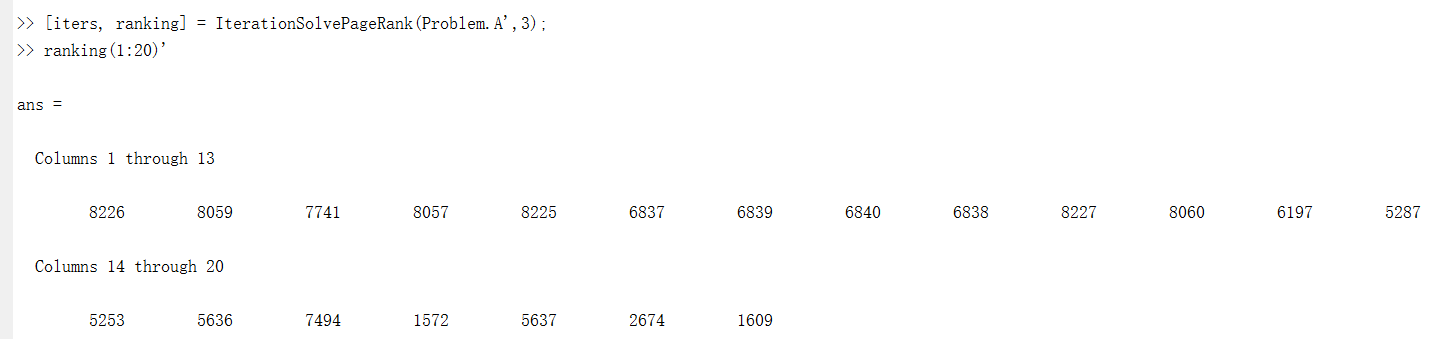
\includegraphics[width=0.8\textwidth]{image/IterationSolvePageRank.png}
		\caption{迭代法运行结果}
		\label{r1}
	\end{figure}
	\begin{figure}[H]
		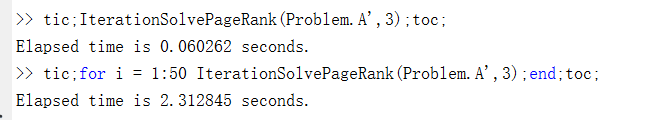
\includegraphics[width=0.8\textwidth]{image/result_ISP.png}
		\caption{运算效率}
		\label{r2}
	\end{figure}
	从图(\ref{r3})中可以看出,在一定误差范围内,迭代法的收敛速度还是很快的,但是到达一定下限后就几乎不会收敛了。
	\begin{figure}[H]
		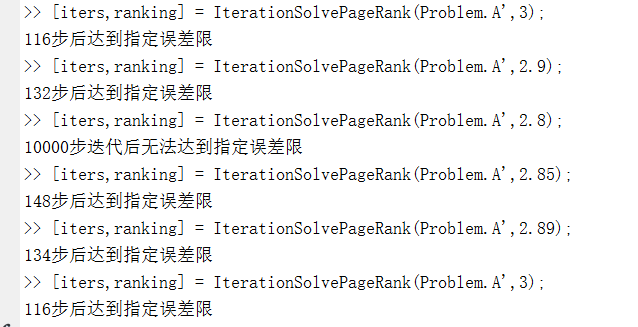
\includegraphics[width=0.8\textwidth]{image/result_ISP1.png}
		\caption{迭代速度}
		\label{r3}
	\end{figure}
	\section{迭代法(归一化)}
	
	\subsection{算法思路}
	如果对上述迭代进行归一化,则会保证有唯一解,但运算结果表明不归一化与归一化结果是一致的。
	\subsection{代码}
	\lstinputlisting{code/IterationSolvePageRank2(UTF8).m}
	\subsection{运行结果}
	可见归一化与没有归一化的结果是一致的。
	\begin{figure}[H]
		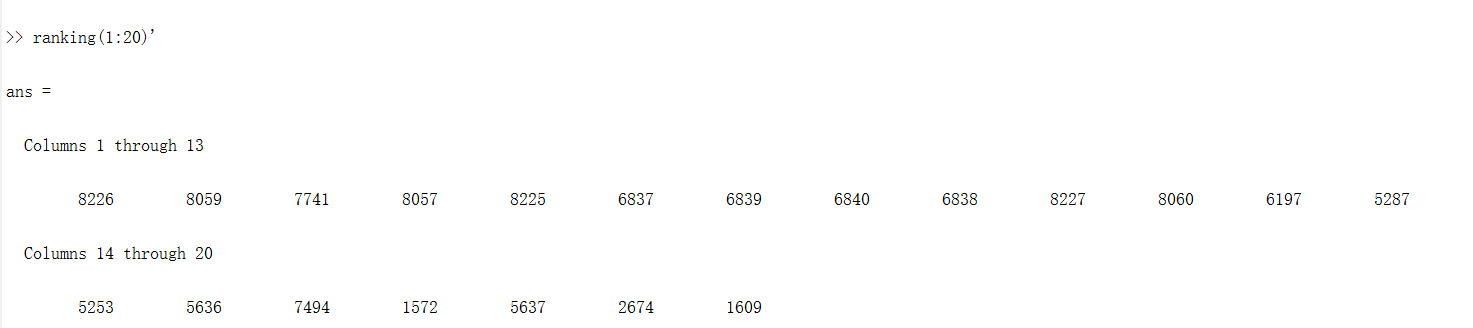
\includegraphics[width=0.9\textwidth]{image/result_ISP2.png}
	\end{figure}
	\begin{figure}[H]
		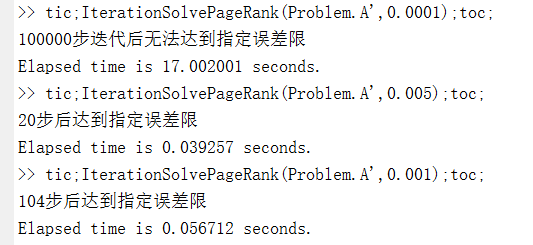
\includegraphics[width=0.9\textwidth]{image/result_ISP3.png}
	\end{figure}
	\section{线性方程组法}
	\subsection{算法思路}
	考虑矩阵 $G = (g_{ij})$,若从网页 $j$ 到 $i$ 有一个链接,则 $g_{ij} = 1$,否则 $g_{ij} = 0$. 记第 $j$ 个网页的出度为
	$c_j = \sum\limits_i g_{ij}$. 将浏览网页视作马尔科夫过程,在浏览网页 $j$ 时,有一定概率选择点击 $j$ 上的链接浏览网页 $i$,也有可能从地址栏或者收藏夹直接切换到网页 $i$. 设浏览 $j$ 时点击其上链接的概率记作 $\rho$ (阻尼因子),网页总量为 $N$,则从网页 $j$ 到网页 $i$ 的转移概率为
	\begin{equation}
	a_{ij} = 
	\left\{
	\begin{array}{lll}
	g_{ij} [\rho\cdot c_{j} + (1 − \rho)\cdot \frac{1}{N} ] + (1 − g_{ij}) [(1 − \rho) \cdot\frac{1}{N} ] = \frac{\rho g_{ij}}{c_j} +\frac{1-\rho}{N}& \text{若}& c_j\neq 0 \\
	\frac{1}{N}& \text{若} & c_j = 0
	\end{array}
	\right.
	\end{equation}
	记 $A = (a_{ij})$,则
	\begin{equation}
	A = \rho GD + ez^T
	\end{equation}
	其中 $D$ 为对角阵$ diag\{d_1, d_2, · · · , d_N\}$,$ e $为行向量 $[1, 1, · · · , 1]$ ,$z$ 为列向量$ [z_1, z_2, · · · , z_N]^T$
	\begin{equation}
	d_j = \left\{\begin{array}{ll}
	0&c_j=0\\
	\frac{1}{c)_j}&c_j\neq 0
	\end{array}
	\right.
	\qquad
	z_j = \left\{
	\begin{array}{ll}
	\frac{1}{N}& c_j=0\\
	\frac{1-\rho}{N}& c_j\neq 0 
	\end{array}
	\right.
	\end{equation}
	于是则有
	\begin{equation}
	Ax = \rho GDx+ez^Tx = x
	\end{equation}
	
	又$z^Tx$的值为定值$k$则
	\begin{equation}
	(I-\rho GD)x = ke
	\end{equation}
	但我们只需要相对大小,所以我们可以将上述方程简化为
	\begin{equation}
	(I-\rho GD)x = e
	\end{equation}
	\subsection{代码}
	\lstinputlisting{code/LinearEqsSolvePageRank.m}
	\subsection{运算结果}
	\begin{figure}[H]
		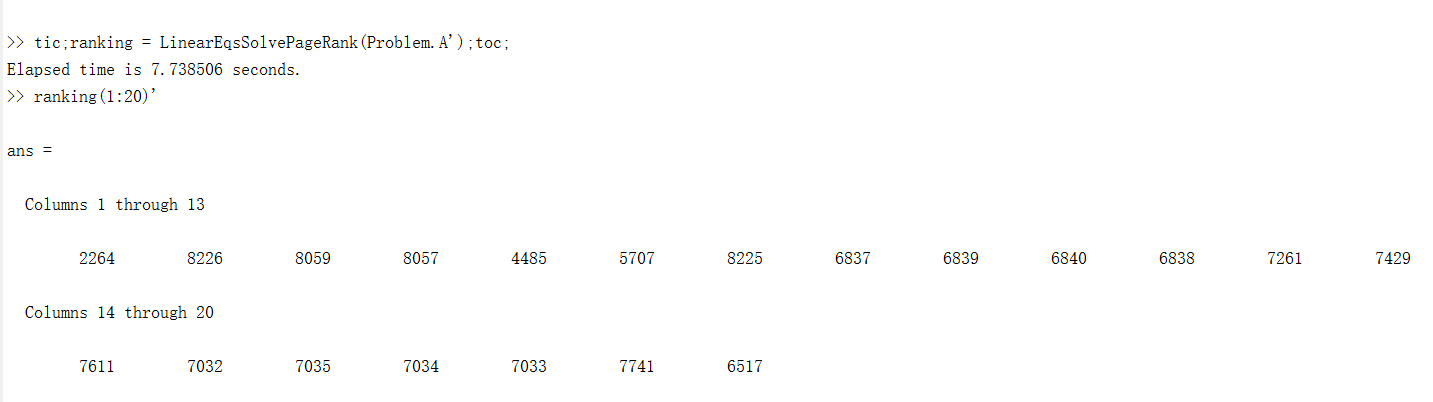
\includegraphics[width=0.9\textwidth]{image/LinearEqsSolvePageRank.png}
		\caption{线性方程组法运行结果}
	\end{figure}
	前十名排序如下图
	
	\begin{figure}[H]				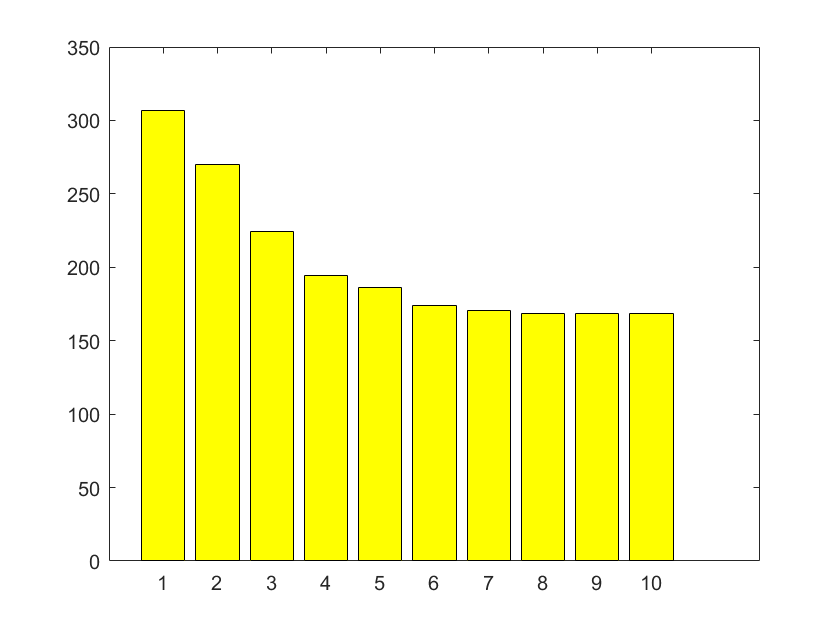
\includegraphics[width=0.8\textwidth]{image/ranking.png}
		\caption{前十名排名}
	\end{figure}
	\section{稀疏矩阵存储}
	\subsection{算法思路}
	对于上述的线性方程组解法,注意到题目提供的矩阵为稀疏矩阵,所以对上述线性方程组的解法中的矩阵用稀疏矩阵存储
	\subsection{代码}
	\lstinputlisting{code/SpLinearEqsSolvePageRank.m}
	\subsection{运行结果}
	运行结果可以发现,运算效率远高于不用稀疏矩阵存储的算法,可见,使用稀疏矩阵不但能够节约内存,还能够加快运算速度。
	\begin{figure}[H]
		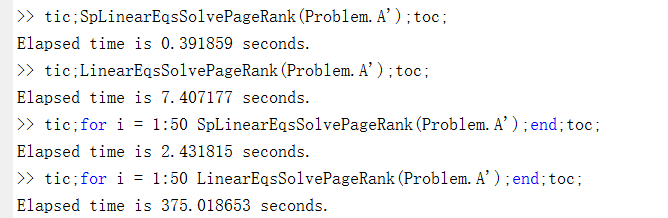
\includegraphics[width=0.8\textwidth]{image/result_sp1.png}
		\caption{稀疏矩阵存储运算效率}
	\end{figure}
	\section{比较与分析}
	对于迭代法和线性方程组法进行 PageRank 排序,前 20 基本相同,但次序不完全一样。但迭代法的收敛速度较小,另外如果进行稀疏存储,则会大大加快运算速度,这在更大规模的网页PageRank的计算中是很有必要的。
	\begin{longtable}{|llll||llll|}
		\hline
		排名&迭代法&迭代法(归一化) & 线性方程组法& 排名&迭代法&迭代法(归一化)&线性方程组法\\
		\hline
		1	&	8226	&	8226		&	2264	&	11	&	8060	&	8060	&	6838	\\
		2	&	8059	&	8059		&	8226	&	12	&	6197	&	6197	&	7261	\\
		3	&	7741	&	7741		&	8059	&	13	&	5287	&	5287	&	7429	\\
		4	&	8057	&	8057		&	8057	&	14	&	5253	&	5253	&	7611	\\
		5	&	8225	&	8225		&	4485	&	15	&	5636	&	5636	&	7032	\\
		6	&	6837	&	6837		&	5707	&	16	&	7494	&	7494	&	7035	\\
		7	&	6839	&	6839		&	8225	&	17	&	1572	&	1572	&	7034	\\
		8	&	6840	&	6840		&	6839	&	18	&	5637	&	5637	&	7033	\\
		9	&	6838	&	6838		&	6840	&	19	&	2674	&	2674	&	7741	\\
		10	&	8227	&	8227		&	6837	&	20	&	1609	&	1609	&	6517	\\
		
		\hline
		\caption{结果比较}
	\end{longtable}
	\end{spacing}
	
\end{document}

